% !TEX root = ../Thesis.tex
\newcommand{\T}{\ensuremath{\mathbf{T}}}
\newcommand{\Tms}{\ensuremath{\T_{\textrm{MS}}}}
\newcommand{\Tid}{\ensuremath{\T_{\textrm{ID}}}}
\newcommand{\C}{\ensuremath{\mathbf{C}}}
\newcommand{\Cms}{\ensuremath{\C_{\textrm{MS}}}}
\newcommand{\Cid}{\ensuremath{\C_{\textrm{ID}}}}
\newcommand{\kt}{\ensuremath{k_{\textrm{T}}}}
\newcommand{\kti}{\ensuremath{k_{\textrm{T},i}}}
\newcommand{\ktj}{\ensuremath{k_{\textrm{T},j}}}
\newcommand{\dij}{\ensuremath{\Delta_{ij}}}
\newcommand{\emissx}[1]{\ensuremath{E^{\textrm{miss,}#1}_{x}}}
\newcommand{\emissy}[1]{\ensuremath{E^{\textrm{miss,}#1}_{y}}}
\newcommand{\emissxy}[1]{\ensuremath{E^{\textrm{miss,}#1}_{x(y)}}}

\chapter{Data Simulation and Object Selection}\label{ch:ObjectSelection}

\section{Monte Carlo simulation}\label{ObjSelMC}

The simulation of data is paramount to HEP research, from the initial detector design phase all the way through to finalized analyses. Monte Carlo (MC) generators simulate various interactions, creating kinematic collision event data that reflect our best understanding of nature. These processes are then passed through detector simulation and all the object reconstruction algorithms, resulting in a dataset with an identical format to collision data. More information on the ATLAS simulation infrastructure can be found in~\cite{Detector:ATLASSimulationInfra}.

The simulation of data happens in three phases: event generation, detector simulation and digitization. 

\subsection{Event generation}\label{ObjSelEventGeneration}

Event generators model complex physics processes that occur during a particle collision. Many different generators exist to model a variety of beam types ($pp$, $p\bar{p}$, $e^+e^-$, etc\ldots) and event types. Hadronic event generators simulate all components of the interaction: the hard scattering process, parton showering, hadronizing, hadronic decay, the underlying event, and photon radiation~\cite{Les}. A schematic diagram of a hadronic event as modelled by an event generator is shown in Figure~\ref{fig:DetectorEGSketch}.

\begin{figure}[p]
  \centering
  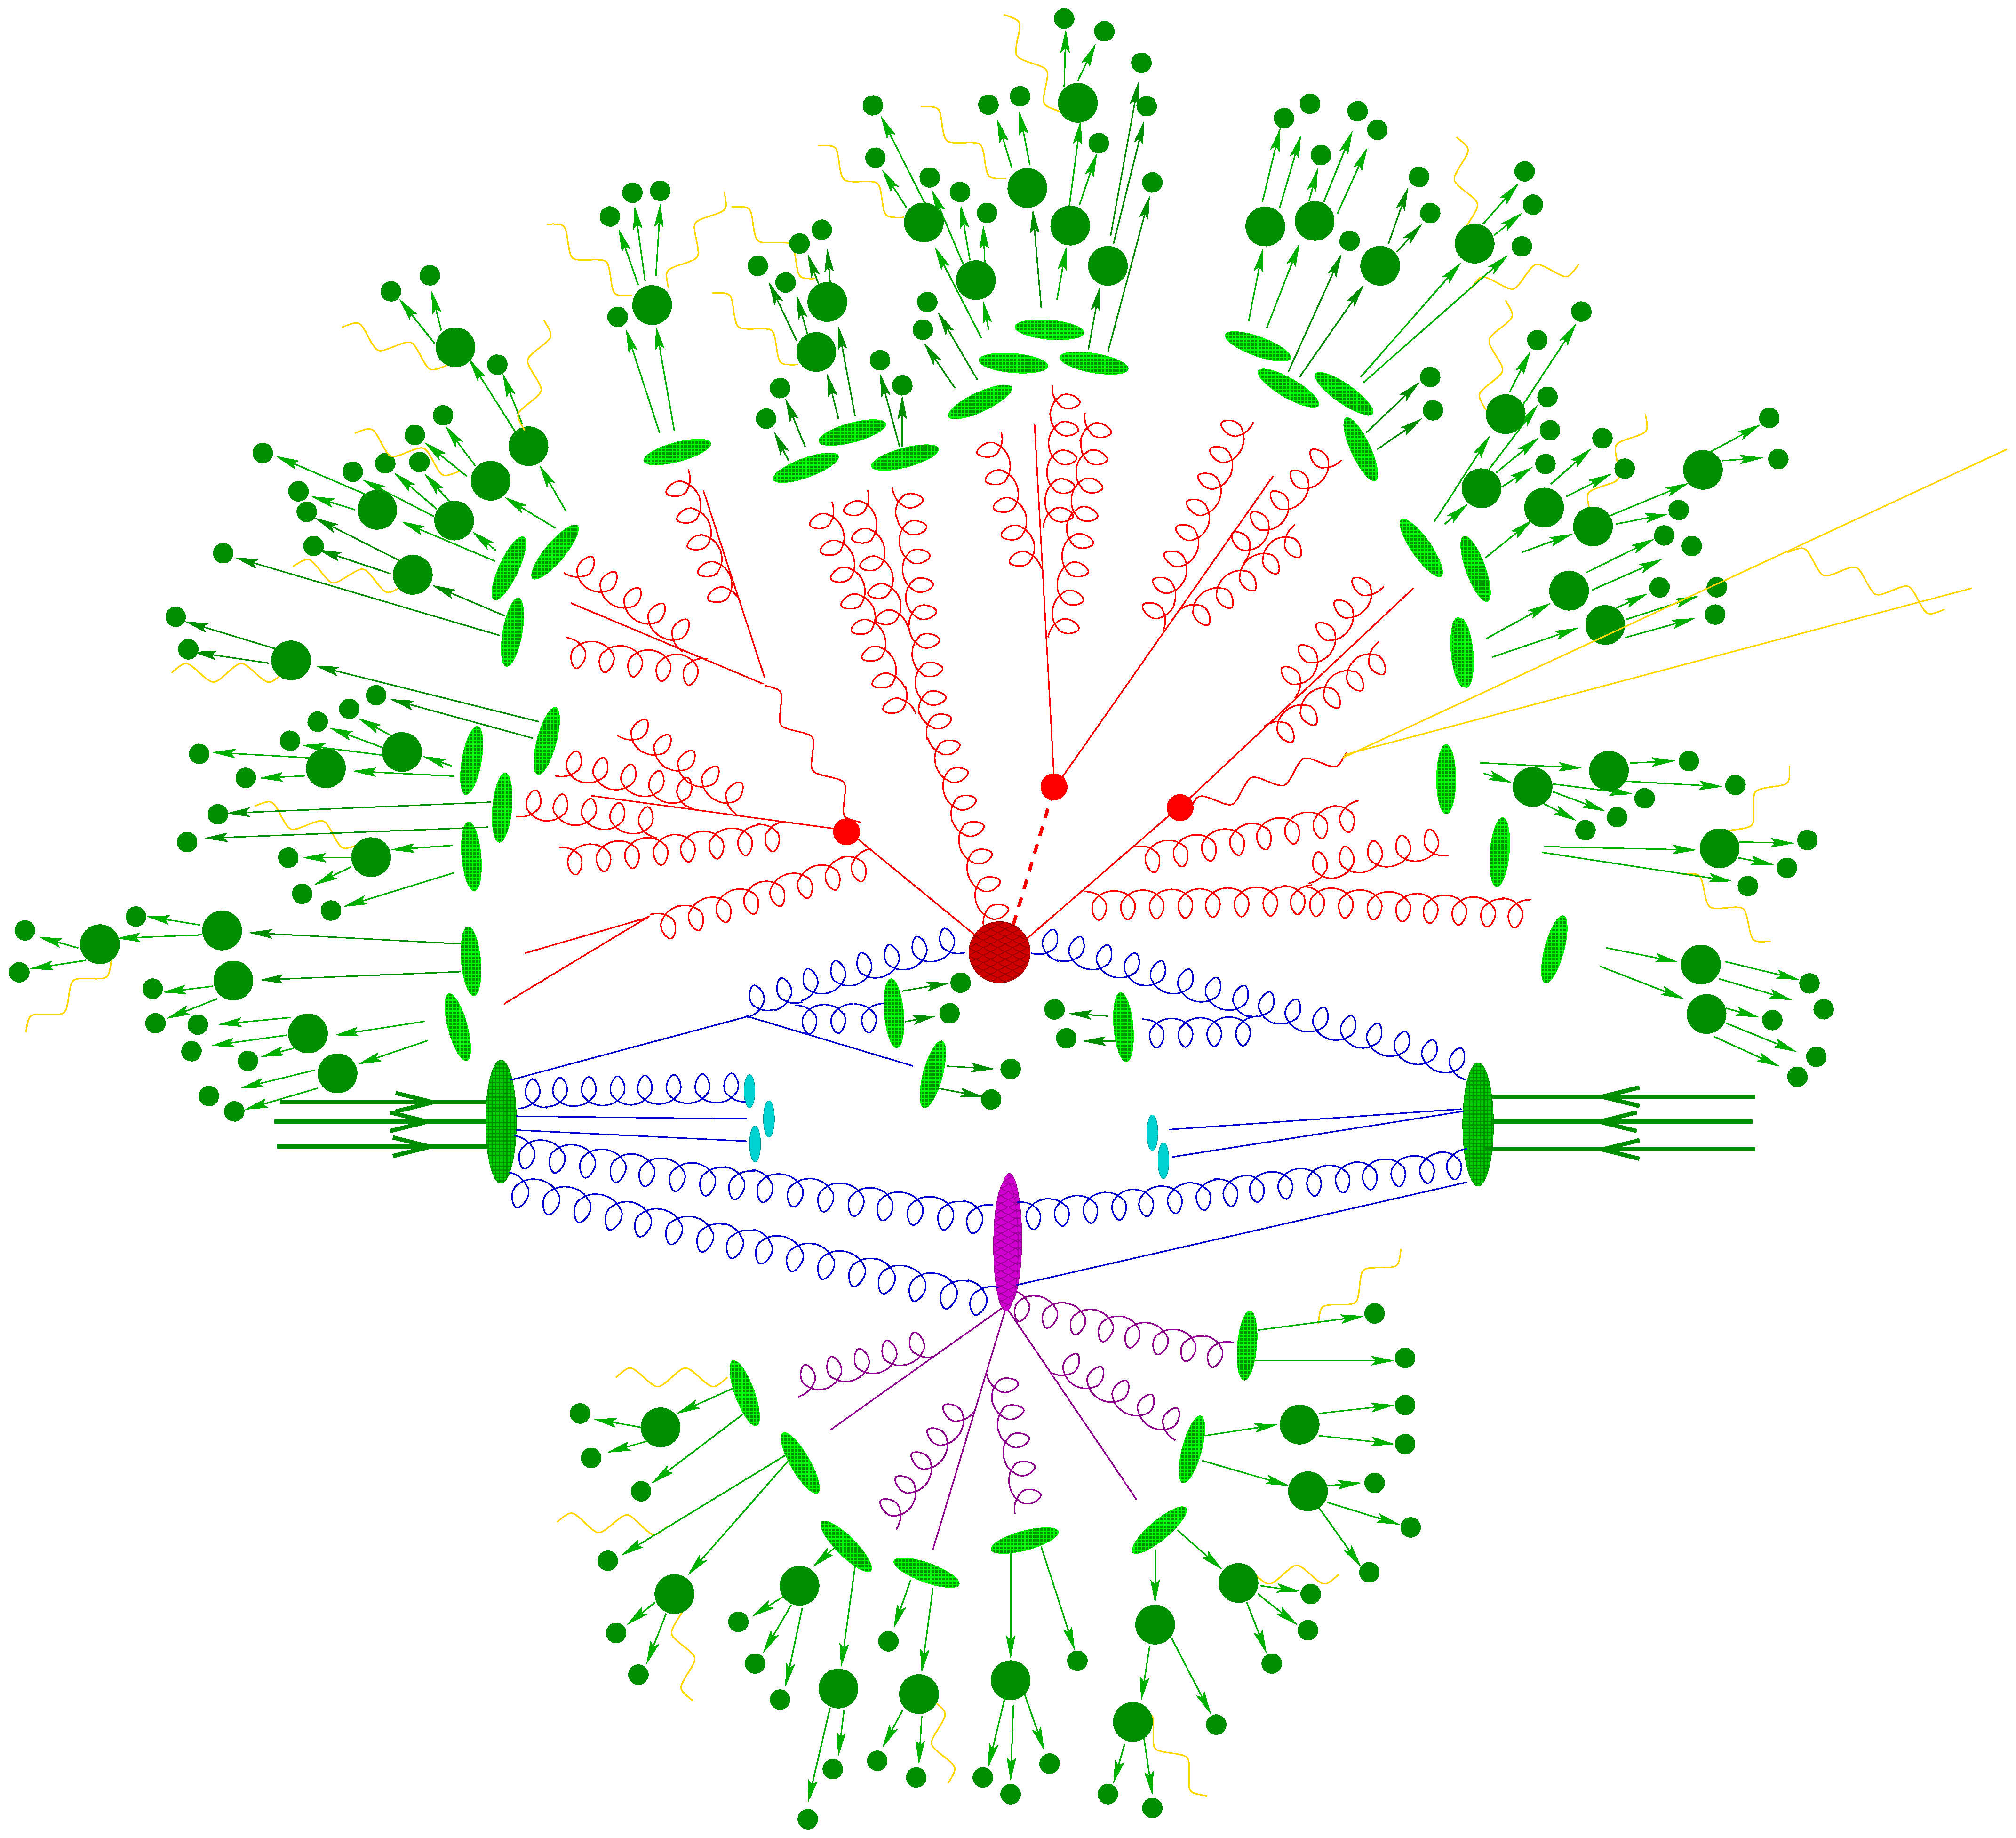
\includegraphics[width=0.90\textwidth]{PartDetector/Diagrams/scetch.eps}
  \caption[Sketch of a proton-proton collision as modelled by the event generator.]{Sketch of a proton-proton collision as modelled by the event generator~\cite{Event}. Shown are the incoming protons beams as green arrows on the left and right sides of the diagram. The partons shown in blue, interact in the hard interaction (red blob) producing a parton shower, also depicted in red, which eventually hadronize (light green blobs) and finally decay into final state particles shown in dark green. The \emph{underlying event} is shown at the bottom of the diagram as the purple blob, note also the beam remnants as light blue blobs that also form part of the underlying event. Photon emission is shown in yellow and occurs at all stages of the event generation.}\label{fig:DetectorEGSketch}
\end{figure}

First, the \emph{hard interaction} of a pair of partons originating from the colliding protons is simulated. An example of such an interaction is $q\bar{q} \rightarrow Z / \gamma^{*}\rightarrow e^{+}e^{-}$. Calculating the cross section for such an interaction involves the convolution of the parton density function (PDF) and the \emph{matrix element} (ME).

The PDF $f_i(x,Q^2)$, describes the probability of finding, within the proton, a parton of flavour $i$ carrying a fraction $x$ of the proton momentum, via a hard interaction with energy scale $Q$. The ME describes the interaction between the two partons and corresponds to one or more of the Feynman diagrams associated with the interaction\footnote{For a rigorous discussion of matrix elements and the Feynman rules, see~\cite{Theory:Perkins,Theory:IntroGriffiths}}. The order of a diagram is determined by the number of coupling constants associated with it. Different generators are capable of treating diagrams at different orders, though the hard interaction is usually modelled at LO or NLO\@.

The next step is \emph{parton-showering} which simulates the emission of gluons by coloured partons and gluon splitting. A cascade of partons is produced, as shown in Figure~\ref{fig:DetectorEGSketch}, and modelled by perturbation theory for energies above \SI{1}{GeV}. All coloured objects are then combined into colourless hadrons in a process known as \emph{hadronization}, these hadrons are subsequently allowed to decay. Finally, the remaining coloured partons not involved in the hard interaction, are allowed to interact forming the \emph{underlying event}. The kinematic information of the original event without the effects of the detector is kept in the data set and is usually referred to as the \emph{truth information}.

\subsection{Detector simulation}\label{sec:DetectorSimulation}

The generated events are then passed through a detector simulation that mimics the response of the detector to particles traversing through it. A description of the entire detector is implemented in the GEANT4 tool-kit~\cite{Detector:Geant4}, including a map of the magnetic fields, the position of the detector components and material description. The software then simulates the signal voltages produced in all tracking and calorimeter components of the detector, these are then passed through a simulation of the read-out electronics and TDAQ taking into account known losses and inefficiencies. All of this information is then passed on to the reconstruction software that ``rebuilds'' the physics objects from the detector hits.

\section{Object reconstruction}\label{sec:DetectorEventReco}

The process of converting the raw data from the detector into physics objects (electrons, muons and so on) is known as \emph{object reconstruction}. The reconstruction algorithms are identical for both collision data and simulated data. As lepton plus jets decays of \ttbar\ are the focus of this thesis, the reconstruction procedures of all types of objects (excluding photons) are relevant. This includes electron, muon and jet reconstruction as well as $b$-tagging algorithms. The soft muon tagger relies on \emph{STACO combined} (STACO CB) muons, therefore some details of the muon reconstruction algorithms are discussed here.

\subsection{Electron reconstruction}\label{sec:DetectorElReco}

The electron reconstruction~\cite{Detector:ElectronReco} procedure at ATLAS depends on the pseudorapidity of the candidate. Only electrons that lie within the coverage of the ID are used here, therefore only the relevant procedure is described. The algorithm used in the central region identifies energy deposits in the EM calorimeter and associates them with reconstructed ID tracks. Firstly, clusters are seeded from energy deposits with total \Et\ above \SI{2.5}{\GeV} using a sliding-window algorithm with window size $3\times5$ in units of $0.025\times0.025$ in ($\eta$,$\phi$) space. Tracks with $\pt>\SI{0.5}{\GeV}$ are then extrapolated to the middle layer of the EM calorimeter\footnote{As it absorbs the largest fraction of the shower energy} and matched to the cluster seed using cuts in the ($\eta$,$\phi$) space. In case of multiple matches, tracks with pixel or SCT hits are given priority and the match with the smallest \DeltaR\ distance is chosen. Finally, the size of the cluster associated with the candidate electron is enlarged to $3\times7$ and $5\times5$ in the barrel and end-cap regions respectively. The energy of the electron is then the sum of four contributions taking into account energy deposited before the EM material, and leakages to other clusters as well as beyond the EM calorimeter.

Electron identification for central electron candidates is done by applying sequential cuts on calorimeter, tracking and combined track-cluster variables. Several sets of selection criteria, labelled \emph{loose}, \emph{medium} and \emph{tight}, are designed for use in analyses. These sets provide increasing background-rejection power at the cost of efficiency by introducing new cuts at each stage, or by tightening previous cuts. The cut definitions are listed in Appendix~\ref{app:DetectorElectronID}.

Additional requirements can be made on the so-called isolation of the electron. Three sets of isolation strategies are used at ATLAS~\cite{Detector:ElectroIsolation}:

\begin{itemize}
  \item \textbf{Calorimeter isolation}: The calorimeter isolation \etcone{\DeltaR}\ is defined as the sum of transverse energy deposited in the cells around the electron in a cone of size \DeltaR. The contribution from the electron itself is removed within $\Delta\eta\times\Delta\phi=0.125\times0.175$ around the electron cluster barycentre. It is corrected for energy leakage from the electron into the isolation cone and for the effect of pile-up. At ATLAS the nominal cone sizes used are $\DeltaR$=\numlist{0.2;0.3;0.4}.
  \item \textbf{Track isolation}: The tracking isolation \nucone{\DeltaR}\ is defined as the number of tracks in a cone around the electron, excluding the track of the electron itself.
  \item \textbf{Momentum isolation}: The momentum isolation \ptcone{\DeltaR}\ is defined by the sum of the transverse momentum of tracks with $\pt>\SI{0.4}{\GeV}$ in a cone around the electron, excluding the electron track itself.
\end{itemize}

\subsection{Muon reconstruction}\label{sec:DetectorMuReco}

Muon reconstruction makes use of the information provided by both the inner detector and the muon spectrometer systems. Several different strategies exist~\cite{Detector:MuonReconstructionList}:

\begin{itemize}
  \item \textbf{Standalone reconstruction}: Uses MS information only, first constructing \emph{segments} from several hits in a given chamber and then fitting segments from all three stations to hits from the four MS components. Tracks are then extrapolated back to the interaction point taking into account energy loss and multiple scattering.
  \item \textbf{Tagging ID tracks reconstruction}: Uses MS or calorimeter information to tag ID tracks as muons.
  \item \textbf{Combined track reconstruction}: Standalone muon tracks are extrapolated back to the vertex and matched to ID tracks within ($\aeta<2.5$) and combined. This results in an improved momentum sensitivity from ID and MS information. 
\end{itemize}

These strategies can be implemented in a variety of ways. There are two prominent families, STACO and MUID, that contain reconstruction packages which exploit one or a combination of these strategies. The STACO combined algorithm is used by the SMT tagger and is described in more detail below.

\subsubsection{STACO Combined algorithm}\label{sec:DetectorSTACO}
The STACO package~\cite{Detector:STACO} combines ID and MS tracks by performing a statistical combination of the two independent tracks using track parameters ($\eta$, $\phi$, \pt, $d_{0}$, and $z_{0}$) and their covariance matrices. The quality of the fit is represented in the resulting \xsm:
%
\begin{equation}
  \xsm = {(\Tms-\Tid)}^T{(\Cms+\Cid)}^{-1}{(\Tms-\Tid)}
  \label{eq:DetectorXsmDef}
\end{equation}
%
where \Tms\ and \Tid\ contain the track parameters for the MS track and the ID track respectively,
% 
\begin{equation}
  \T_{\textrm{MS or ID}} =
  \begin{pmatrix}
    \eta \\
    \phi \\
    \pt \\
    d_{0} \\
    z_{0}
  \end{pmatrix}
\end{equation}
%
and \Cms\ and \Cid\ are the covariance matrices, defined as
%
\begin{equation}
  \C_{ij} = {(\T_i-\langle \T_i\rangle)}{(\T_j-\langle \T_j\rangle)}
\end{equation}
%
where $\langle \T_i\rangle$ is the expectation value of $\T_i$. The full covariance matrix is shown in Appendix~\ref{app:DetectorCov}.

If more than one possible combination per track exists, the best combined \xsm\ is chosen and then the track is removed from the pool of tracks to be matched. The algorithm continues making associations until no more tracks remain.

Finally, tracking, calorimeter and momentum isolation variables are defined in a similar way as with electrons.

\subsubsection{MUID algorithm}\label{sec:MUID}

The MUID reconstruction package~\cite{Detector:ExpectedPerf} implements all muon reconstruction strategies described before. The MUID standalone (SA) algorithm uses tracks and segments reconstructed at the muon spectrometer by the Moore algorithm~\cite{Detector:MooreReconstruction}, and extrapolates inwards to obtain track parameters at the vertex. The MuGirl algorithm~\cite{ObjSelection:MuGirl} searches for MS tracks and segments using an ID track as a seed. If the full track refit is successful a combined muon is made, otherwise a tagged muon is made. The MUID family also contains a combined muon algorithm that use a global fit of the tracks reconstructed in the ID and in the MS\@.

\subsection{Jet reconstruction}\label{sec:Detector-JetReconstruction}

As quarks and gluons hadronize and fragment they produce a large number of soft hadrons and high energy photons. This process results in an object known as a ``jet''. A jet reconstruction algorithm attempts to recombine all these components to reconstruct the four-momentum vector of the original quark/gluon. The reconstructed jets are the closest physical representation of a hard quark or a gluon available to experimentalists. The development of jet reconstruction algorithms is driven by theoretical and experimental requirements. From a theoretical perspective, it is crucial that jet algorithms be \emph{infra-red and collinear} (IRC) safe. The probability of gluon emission approaches infinity in the collinear and soft regime. These infinities cancel out with virtual gluon emission. If jets resulting from hard particles are merged or split due to soft emission or collinear splitting these probabilities do not cancel and a divergence occurs. A jet algorithm is said to be IRC safe when the reconstructed jets remain unchanged under the addition of a soft emission or a collinear splitting. Jet algorithms should also be able to work given parton, hadron, or calorimeter information. From an experimental perspective, jet algorithms should be stable under increased luminosity or centre of mass energy, be computationally efficient and fast, and work independently of detector technology. 

There are many different jet reconstruction algorithms such as the Cambridge/Aachen, \kt\ and SISCone, however only the ATLAS default known as the anti-\kt\ algorithm is used here.

\subsubsection{Anti-\kt\ algorithm}

The anti-\kt\ algorithm is a clustering algorithm that sequentially combines objects to form cone-shaped jets~\cite{Cacciari:2008gp}. This algorithm has been found to be more resilient to the effects of pile-up and underlying event, and the shape of the jet is unaffected by soft radiation producing circular jets. It is also computationally efficient and fast given a smart implementation~\cite{Detector:FastJetKt}.

The clustering process begins by measuring two distances: the distance between all particles $d_{ij}$, and the distance between particle $i$ and the beam $d_{iB}$ defined as
%
\begin{align*}
    d_{ij} &= \textrm{min}(\kti^{-2}, \ktj^{-2})\frac{\Delta_{ij}^2}{R^{2}} \\
    d_{iB} &= \kti^{-2}
\end{align*}
%
where $\dij^2={(y_i-y_j)}^2+{(\phi_i-\phi_j)}^2$, and \kti, $y_{i}$ and $\phi_{i}$ are the transverse momentum, rapidity, and azimuthal angle of object $i$. The parameter $R$ defines the characteristic cone size of the jet, note that by construction not all anti-\kt\ jets are conical. For every object both distances are calculated, if $d_{ij}$ is the smallest then objects $i$ and $j$ are combined forming proto-jets, if $q_{iB}$ is smallest the object is labelled as a final jet and removed from the list of objects to be combined. This process continues until all objects are removed. 

In general, soft particles will tend to combine with hard objects before combining with other soft objects. If two hard objects lie at $2R$ from each-other, they will both form conical shapes with radius $R$. Otherwise partially conical jets will form depending on the relative magnitudes of \kt\ of each particle. The standard value of $R$ used for ATLAS analyses is $0.4$, this is used here unless stated otherwise.

\subsubsection{Jet calibration}

The process of jet calibration corrects the jet energy as measured in the detector with the intention of recovering the energy of the original stable particle jet that entered the detector. Clusters of energy deposits in the calorimeter, known as topo-clusters, are constructed from topologically connected calorimeter cells~\cite{Detector:JetEnergyMeasurement}. Calorimeter jets are constructed from topo-clusters that enter the clustering algorithm as massless particles. 

These clusters are initially reconstructed at the EM scale, which correctly measures the energy of particles in EM showers. If jet reconstruction is carried on these clusters the jets are known as EM jets. An additional collection of topo-clusters is created by calibrating the calorimeter cells to correctly reconstruct the response of the calorimeter to hadrons. The main calibration scheme is known as \emph{local cluster weighting} (LCW)~\cite{Detector:JetEnergyMeasurement}. In this scheme each topo-cluster is classified as electromagnetic or hadronic based on shower shape variables, then simulation-derived corrections are applied to each cluster. These correct for the effects of non-compensation, signal losses due to threshold effects, and energy loss in non-instrumented regions of the calorimeter. These corrected topo-clusters are then used in the jet reconstruction algorithms, to build LCW jets. 

Additional corrections are applied to topo-clusters at either EM or LCW scale in an attempt to restore the \emph{jet energy scale} (JES) to that of jets reconstructed from simulated stable particles. Additional corrections are applied to compensate for the effects of pile-up, align the jet to point to the primary vertex rather than the ATLAS centre, and other corrections derived from MC simulations. Jets corrected in this way are said to be at the EM+JES scale or LCW+JES scale depending on the scale of the topo-clusters. Each calibration methodology has some uncertainties associated with it, which vary with jet \pt\ and $\eta$~\cite{Detector:JESPaper}.

\subsection{\texorpdfstring{$b$}{b}-jet tagging techniques}

Identification of heavy flavour (HF) jets, from $b$- or $c$-quarks, is very important in the study of many types of events including \ttbar\ events. Identification of $b$-jets is generally known as $b$-tagging. Many $b$-taggers have been developed at ATLAS to achieve the highest efficiency along with strong rejection of LF jets. These algorithms exploit a variety of strategies including impact parameters (IP3D), secondary vertex reconstruction (SV1) and the topology of the $b$- and $c$-hadron decays (JetFitter). The output of these variables are used as inputs into multivariate algorithms to provide enhanced $b$-tagging capabilities. The default algorithm at ATLAS is known as the MV1 tagger is one such algorithm. Finally, \emph{soft lepton tagging} (SLT) exploits the production of leptons within some $b$-jets to provide separation from LF. The performance of these $b$-taggers is shown in Figure~\ref{fig:DetectorTaggingPerf}. The tagger used in this thesis is an implementation of soft lepton tagging described in more detail below.

\begin{figure}[htbp]
  \centering
  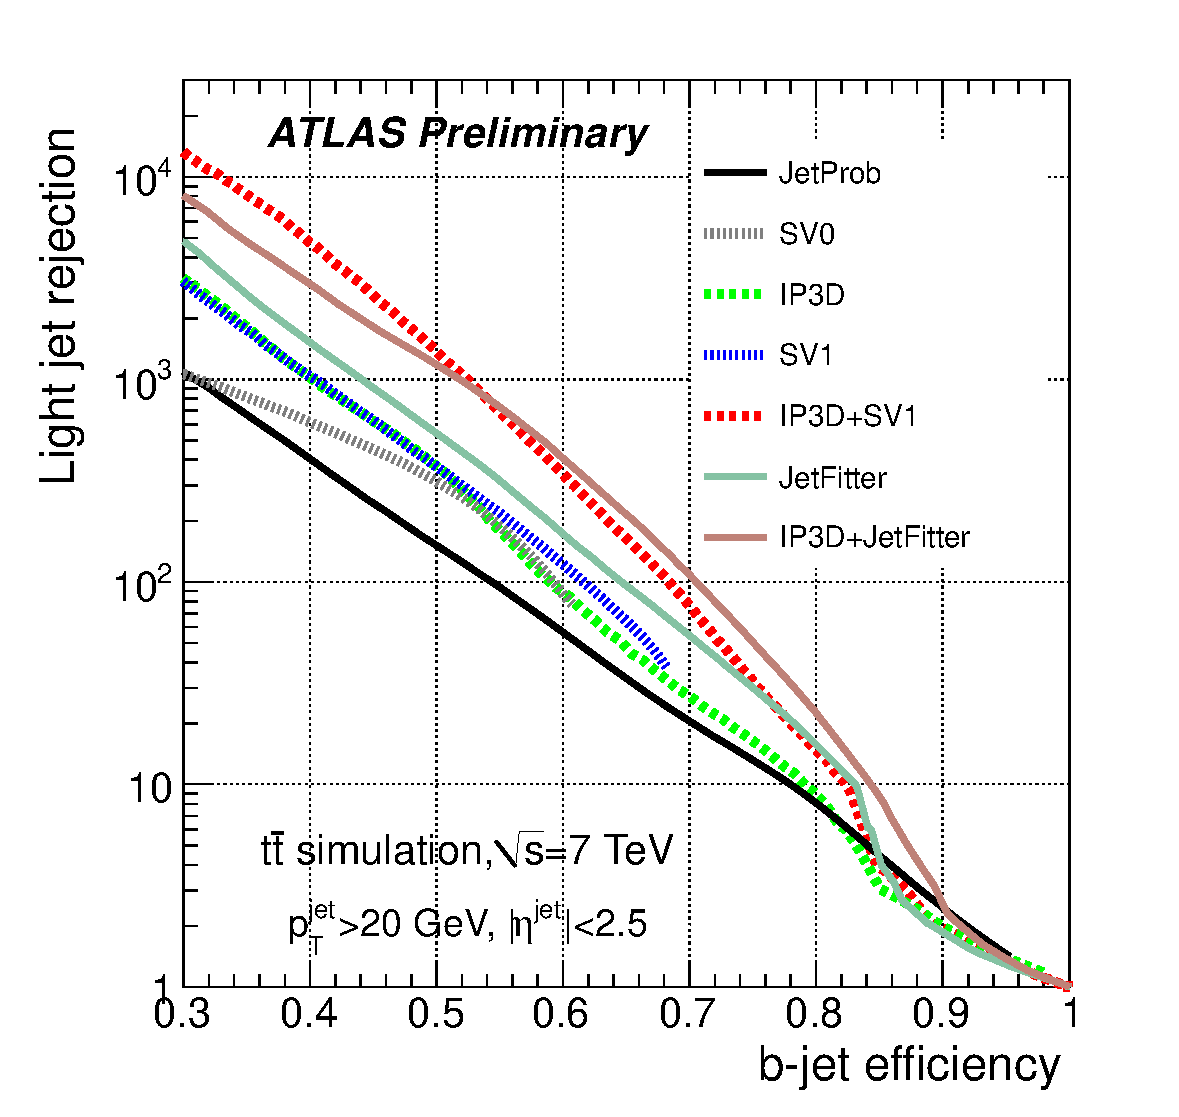
\includegraphics[width=0.75\textwidth]{PartDetector/Plots/DetectorBtaggingPerformanceComp.eps}
  \caption[Light jet rejection as a function of the $b$-jet tagging efficiency, comparing some of taggers used at ATLAS as measured in simulated \ttbar\ events.]{Light jet rejection as a function of the $b$-jet tagging efficiency, comparing some of taggers used at ATLAS as measured in simulated \ttbar\ events~\cite{Detector:TaggingJetFitter}.}\label{fig:DetectorTaggingPerf}
\end{figure}

\subsubsection{The SV0 and SV1 algorithms}

The SV0 algorithm~\cite{Detector:BTaggingSV0} reconstructs secondary vertices using tracks within the cone of the candidate jet. These secondary vertices are located at a decay length $L$ from the primary vertex. A cut is then applied on the decay length significance $L/\sigma_{L}<5.72$, this is an operating point that yields a $b$-tagging efficiency of $\SI{50}{\percent}$ as measured on simulated inclusive \ttbar\ events.

The SV1 algorithm is an extension of the SV0 algorithm. In order to improve the tagging performance, three properties of the secondary vertex are used as inputs to a likelihood ratio: the invariant mass of the tracks associated to the vertex, the ratio of the sum of the energies of the tracks in the vertex to the sum of the energies of the tracks in the jet, and the number of two-track vertices. The $\DeltaR$ between the jet axis and the line joining the primary and secondary vertices is also used.

\subsubsection{The JetFitter algorithm}

The JetFitter algorithm~\cite{Detector:TaggingJetFitter} uses a Kalman filter to find a line along which the $b$ quark, $c$ quark, and the primary vertices lie along with their position on the line, giving an approximated flight-path for the $B$-hadron. Discrimination is based on a likelihood using similar variables as in the SV1 algorithm and variables such as the flight length significances of the secondary vertices.

\subsubsection{The IP3D algorithm}

The IP3D algorithm makes use of the transverse and longitudinal impact parameter significances in two-dimensional histograms to discriminate between $b$, $c$ and LF jets. A likelihood-ratio method is used: the IP significances are compared to pre-defined smoothed and normalized distributions for $b$- and light-jets hypotheses. This produces a weight distribution for each model and a cut is applied to select jets. The IP3D algorithm is often combined with the JetFitter (IP3D+JetFitter) or SV1 algorithm (IP3D+SV1) to provide additional discriminating power.

\subsubsection{The MV1 algorithm}

The MV1 algorithm uses the output weights of the IP3D, SV1 and JetFitter algorithms as inputs to an artificial neural network. The working point used at ATLAS is defined so as to achieve a $b$-tagging efficiency of \SI{70}{\percent} with an associated mistag rate of less than \SI{1.5}{\percent}~\cite{DetectorBtaggingMistagMV1} depending on the pseudorapidity and transverse momentum of the jet in question. Note that this efficiency is not constant with respect to the jet \pt\ as can be seen from Figure~\ref{fig:DetectorMV1Perf}. The performance at low \pt\ degrades as the decay length is shorter so finding the secondary vertex is more difficult.

\begin{figure}[htbp]
  \centering
  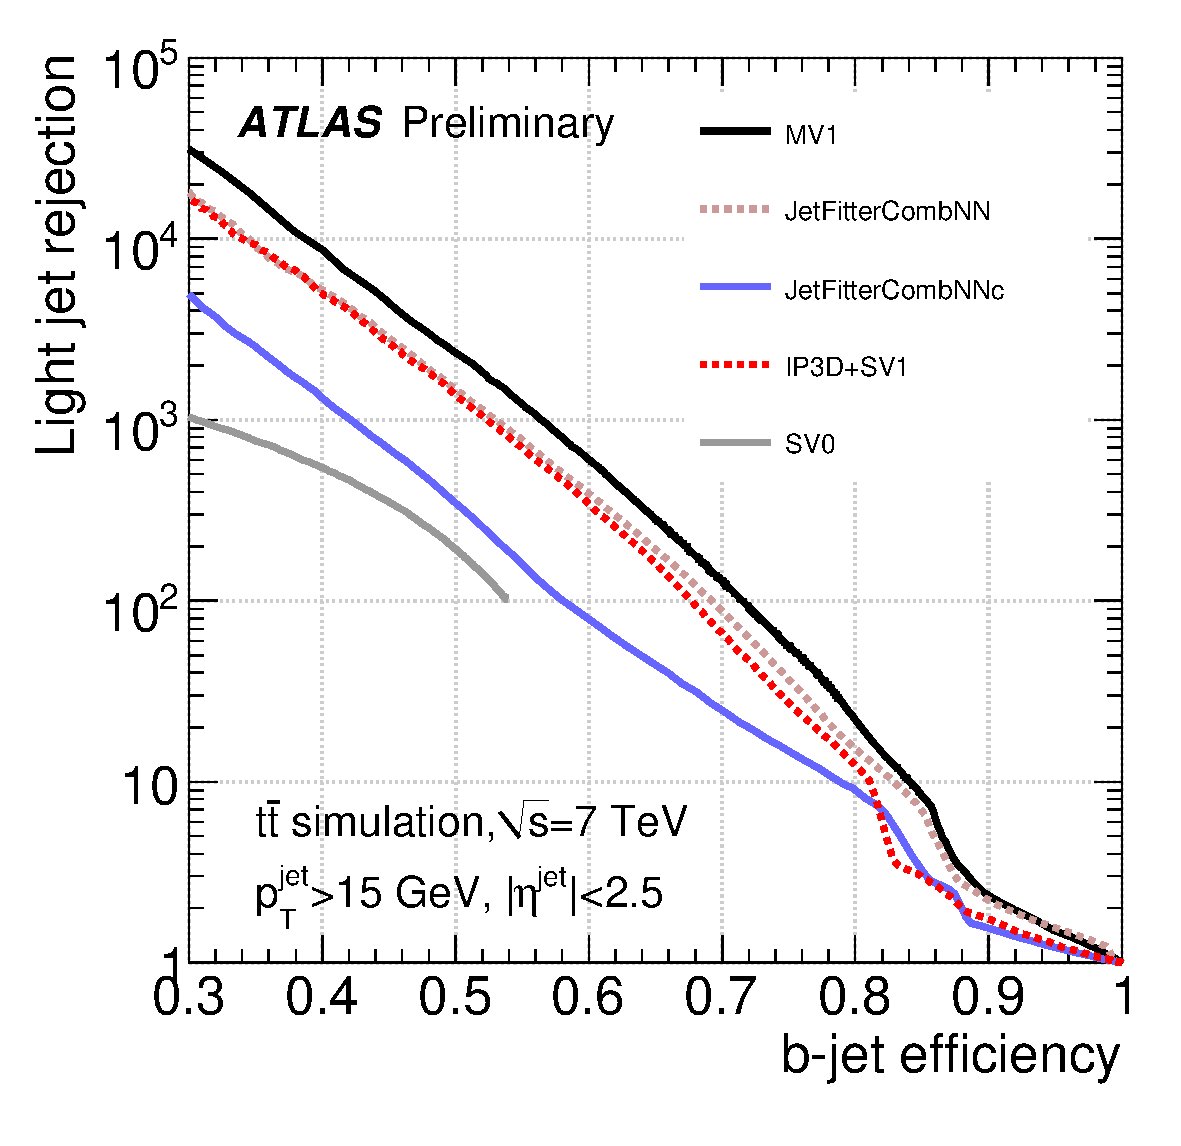
\includegraphics[width=0.75\textwidth]{PartDetector/Plots/MV1Perf.pdf}
  \caption[The light jet rejection factor as a function of $b$-tagging efficiency as measured in simulated \ttbar\ events for the MV1, SV0, IP3D+SV1, and the JetFitterCombNN taggers.]{The light jet rejection factor as a function of $b$-tagging efficiency as measured in simulated \ttbar\ events for the MV1, SV0, IP3D+SV1, and the JetFitterCombNN taggers~\cite{Detector:MV1TaggerEffs}.}\label{fig:DetectorMV1Perf}
\end{figure}

\subsubsection{Soft lepton tagging}\label{sec:DetectorSLT}

\emph{Soft lepton tagging} (SLT) algorithms attempt to identify leptons produced in the semileptonic decay of $b$ and $c$ quarks for the purpose of determining the presence of HF quarks. The term ``semileptonic'' here refers to the decay of a $B$-hadron in such a way as to produce a lepton-neutrino pair with an additional hadron. The lepton produced is known as a \emph{soft} lepton due to its relatively low transverse momentum.

A soft muon can be produced in a variety of ways starting from a $b$-quark, either directly via $b\rightarrow \mu\bar{\nu}_{\mu}X$, where $X$ is any hadron; or indirectly, via a $c$, $\bar{c}$ or a $\tau$ lepton. The direct and indirect via a $c$ production mechanisms are shown in Figure~\ref{fig:DetectorSLTFeynm}. The branching ratio for each of these decays is shown in Table~\ref{tab:DetectorSLTBR}. The total BR for the production of a soft muon from a $b$ quark is \SI[multi-part-units=single]{20.1(10)}{\percent}, thus the probability for a \ttbar\ event to contain at least one semileptonic $b$ decay is approximately \SI{36}{\percent}.

\begin{figure}[htbp]
  \centering
    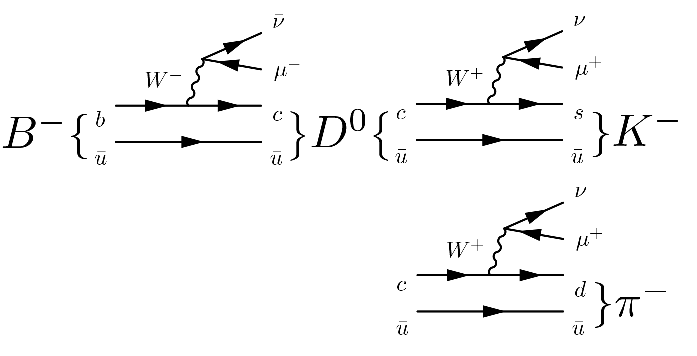
\includegraphics[width=0.75\textwidth]{PartDetector/Diagrams/SemiLeptonicDecay.pdf}
    \caption[Feynman diagram of one of the mechanisms for lepton production via semileptonic $b$ decay.]{Feynman diagram of one of the mechanisms for lepton production via semileptonic $b$ decay. Shown are the direct $b\rightarrow \mu$ and indirect $b\rightarrow c\rightarrow\mu$.}\label{fig:DetectorSLTFeynm}
\end{figure}

\begin{table}[htbp]
  \centering
    \begin{tabular}{@{}lS[table-format=2.2(2)]@{}}
      \toprule
      Mode                                        & {Muon BR [\si{\percent}]} \\
      \midrule % -------------------------
      $b\rightarrow \mu^{-}$                      & {$\num{10.95}\;^{+\;0.29}_{-\;0.25}$} \\
      $b\rightarrow c \rightarrow \mu^{+}$        & 8.02(19) \\
      $b\rightarrow \bar{c} \rightarrow \mu^{-}$  & 1.6(5) \\
      $b\rightarrow \tau^{-} \rightarrow \mu^{-}$ & 0.42(4) \\
      \midrule % -------------------------
      All modes                                   & 21.0(10) \\
      \bottomrule % -------------------------
    \end{tabular}
    \caption[Branching ratio for the production of a muon from a $b$-quark in both direct and indirect modes.]{Branching ratio for the production of a muon from a $b$-quark in both direct and indirect modes~\cite{Theory:PDGBooklet}.}\label{tab:DetectorSLTBR}
\end{table}

The soft muon tagger used in this analysis is based on the quality of the fit between the ID track and MS track as represented by the \xsm. Several tagger-specific cuts (summarized in Table~\ref{tab:DetectorSMTCuts}) are placed on the candidate muons and jets. Candidate SMT muons are required to lie within the coverage of the ID and have sufficient transverse momentum for reliable reconstruction. Requirements are made on the impact parameters of the muon ID track to remove contributions from spurious matches between ID and MS tracks, and from pile-up vertices. Finally, the main cut on the quality of the fit $\xsd=\xsm/\ndof$ is set at less than \num{3.2}. This is an operating-point that provides a $b$-jet (semileptonic $b$-jet) identification efficiency of \SI{10}{\percent} (\SI{50}{\percent}) and a LF rejection factor of 200 per jet. Candidate jets are required to have more than three charged tracks associated with them or a jet EM fraction smaller than \num{0.8}. These criteria ensure that the jet did not originate from the muon itself. Finally, the muon is associated to the jet with a cut $\DeltaR_{\mu}^{\textrm{jet}}<0.5$. The following chapter describes the calibration of the SMT tagger.

\begin{table}[htbp]
\ra{1.2}
  \centering
  \begin{tabular}{ll}
  \toprule
  \multicolumn{2}{c}{\textbf{Muon cuts}} \\
  \midrule
  Muon to jet association & $\DeltaR_{\mu}^{\textrm{jet}}<0.5$ \\
  \multirow{2}{*}{Reconstruction} & $|\eta|<2.5$ \\
                                  & $\pt>\SI{4}{GeV}$ \\
  \multirow{2}{*}{Pile-up reduction} & $|d_0|<\SI{3}{\mm}$ \\
                         & $|z_0\sin{\theta}|<\SI{3}{\mm}$ \\
  Track matching quality & $\xsd<3.2$ \\
  \midrule
  \multirow{2}{*}{Muon-jet rejection} & Jet $N^{\textrm{charged}}_{\textrm{trk}} > 3$ \textbf{or} \\
    & $\textrm{Jet EM fraction} < \num{0.8}$ \\
  \bottomrule
  \end{tabular}
  \caption{Jet and muon SMT Cuts.}\label{tab:DetectorSMTCuts}
\end{table}

\subsection{Missing energy reconstruction}

Missing energy is reconstructed by combining information from energy depositions in the calorimeter, as well as information from the muon spectrometer~\cite{Detector:METReco}. An energy imbalance in the detector is then treated as missing energy.
The two components of the vector $\bm{E}_{\textrm{T}}^{\textrm{miss}}$ are calculated thus:

\begin{equation}
  E^{\textrm{miss}}_{x(y)} = \emissxy{\textrm{calo}} + \emissxy{\mu}
\end{equation}

ID tracking information is used to recover low-\pt\ that are missed in the calorimeters, and for muons in regions not covered by the MS\@. The magnitude of the missing energy \met, which is normally used in event selections, are calculated as:

\begin{equation}
  \met = \sqrt{{(E^{\textrm{miss}}_{x})}^2 + {(E^{\textrm{miss}}_{y})}^2}
\end{equation}

The calorimeter term is constructed by associating calorimeter cells with reconstructed and identified high-\pt\ objects in order: electrons, photons, hadronically decaying $\tau$-leptons, jets, and muons. Calorimeter cells not associated are also included in the summation as \emissxy{\textrm{CellOut}}. Thus each components of the calorimeter term of the missing energy are the linear sum of each contribution:
%
\begin{equation}
  \emissxy{\textrm{calo}} = \emissxy{e} + \emissxy{\gamma} + \emissxy{\tau} + \emissxy{\textrm{jets}} + \emissxy{\textrm{softjets}} + \emissxy{\textrm{CellOut}} + (\emissxy{\mu})
\label{eq:SelectionETMissCalo}
\end{equation}
%
where the muon term is not always added~\cite{Detector:METReco}.

Each component is calculated as the negative sum of calibrated cell energies for each corresponding object, as:

\begin{align}
  \emissx{\textrm{term}} &= -\sum_{i=1}^{N_{\textrm{cell}}^{\textrm{term}}} E_{i}\sin{\theta_{i}}\cos{\phi_{i}} \\
%
  \emissy{\textrm{term}} &= -\sum_{i=1}^{N_{\textrm{cell}}^{\textrm{term}}} E_{i}\cos{\theta_{i}}\sin{\phi_{i}}
\end{align}
%
where $E_{i}$, $\theta_{i}$, and $\phi_{i}$ are the energy and angular position of the cell.

The muon term of the missing transverse energy is calculated as the negative sum of the momenta of muon tracks reconstructed in $|\eta|<2.7$:

\begin{equation}
  \emissxy{\mu} = -\sum_{\textrm{muons}} p^{\mu}_{x(y)}
\end{equation}

For muons in the region covered by the ID, only combined muons are considered to remove contributions from fake muon sources such as energetic hadrons that ``punch through'' the calorimeter. In this region, muons which are well separated from jets, $\DeltaR>0.3$, are treated separately from muons which are non-isolated:

\begin{itemize}
  \item \textbf{Isolated muons:} The combined track \pt\ corrected for energy losses in the calorimeter is used the summation. The muon calorimeter energy term is not included to avoid double-counting.
  \item \textbf{Non-isolated muons:} The muon momentum as measured in the spectrometer after energy loss is used. The muon term \emissxy{\mu}\ is then added to the calorimeter term in Equation~\ref{eq:SelectionETMissCalo}.
\end{itemize}

Outside of the coverage of the ID ($2.5<|\eta|<2.7$) there is no combined track requirement and the \pt\ as measured in the MS is used for both isolated and non-isolated muons. For more information on the measurement and calibration of \met\ at ATLAS see~\cite{Detector:METReco}. 
